\chapter{Persistierung} % (fold)
\label{cha:persistierung}

In den vorangegangen drei Kapiteln wurde die Umsetzung des eigentlichen Werkzeugs beschrieben. Neben der Unterstützung des Modellierungsvorgangs ist aber auch die persistente Speicherung der erstellten Modelle zum Zwecke der Weiterverarbeitung ein hier zu beleuchtender Aspekt. Auf die Persistierung wirken vor allem zwei der in Kapitel XY identifzierten Anforderungen ein. Zum ersten ist die Nachvollziehbarkeit des Modellierungsvorganges sicherzustellen -- dies gilt nicht nur während des Vorgangs selbst, sondern auch danach. Dementsprechend ist sämtliche Information zu persistieren, die zur Wiederherstellung nicht nur des Modells selbst sondern auch der gesamten Modellierungshistorie notwendig ist. Zum zweiten hat die Forderung nach semantischer Offenheit bei der Modellierung auch unmittelbare Auswirkungen auf die Persistierung. Neben dem Modell selbst muss aufgrund dieser Anforderung auch die Bedeutung der verwendeten Modellierungselemente miterfasst und persistiert werden, so dass diese bei der Weiterverarbeitung der Modelle verwendet werden kann.

In diesem Kapitel werden nun aufgrund der eben genannten Forderungen technologische Ansätze identifiziert, beschrieben und schließlich hinsichtlich ihrer Eignung für den konkreten Einsatz beurteilt. Der ausgewählte Ansatz wird im darauf folgenden Abschnitt konzeptuell beschrieben. Die Abbildung der Modelle und der ebenfalls zu persistierenden zusätzlichen Information in ein geeignetes Datenmodell ist Gegenstand des darauf folgenden Abschnitts. Schließlich wird die konkrete technische Umsetzung der Persistierung dargelegt und die dazu notwendigen Software-Module im Detail beschrieben.
 
\section{Möglichkeiten der Persistenzsicherung} % (fold)
\label{sec:möglichkeiten_der_persistenzsicherung}

\begin{itemize}
	\item Serialisierung von Java-Objekten
	\item Relationale Datenbanken
	\item XML Topic Maps
\end{itemize}

% section möglichkeiten_der_persistenzsicherung (end)

\section{Topic Maps} % (fold)
\label{sec:topic_maps}

Topic Maps \citep{TMDM08} sind wie bereits in Abschnitt XY beschrieben ein Mittel zur Abbildung von semantischen Netzen. In Topic Maps können beliebige Daten strukutriert aufbereitet und zueinander in Beziehung gesetzt werden. Die Art der zu repräsentierenden Daten ist dabei irrelvant, eine Topic Map trifft keine Aussage über ein den repräsentierten Daten zugrundeliegendes Begriffsystem (sie ist „ontology-agnostic“ \citep{Vatant04}).

Historisch stammen Topic Maps aus dem Bereich der technischen Repräsentation von Thesauri und Indizes \citep{Pepper00} \citep{Rath03}. Aus diesen Bereichen motivieren sich auch die Bausteine einer Topic Map, wenngleich der Verwendung durch diesen Ursprung nicht eingeschränkt wird. Die grundlegenden Elemente einer Topic Map sind „Topics“, „Associations“ und „Occurrences“ (siehe Abbildung \ref{fig:img_Persistenz_TMBasic}). 

\begin{figure}[htbp]
	\centering
		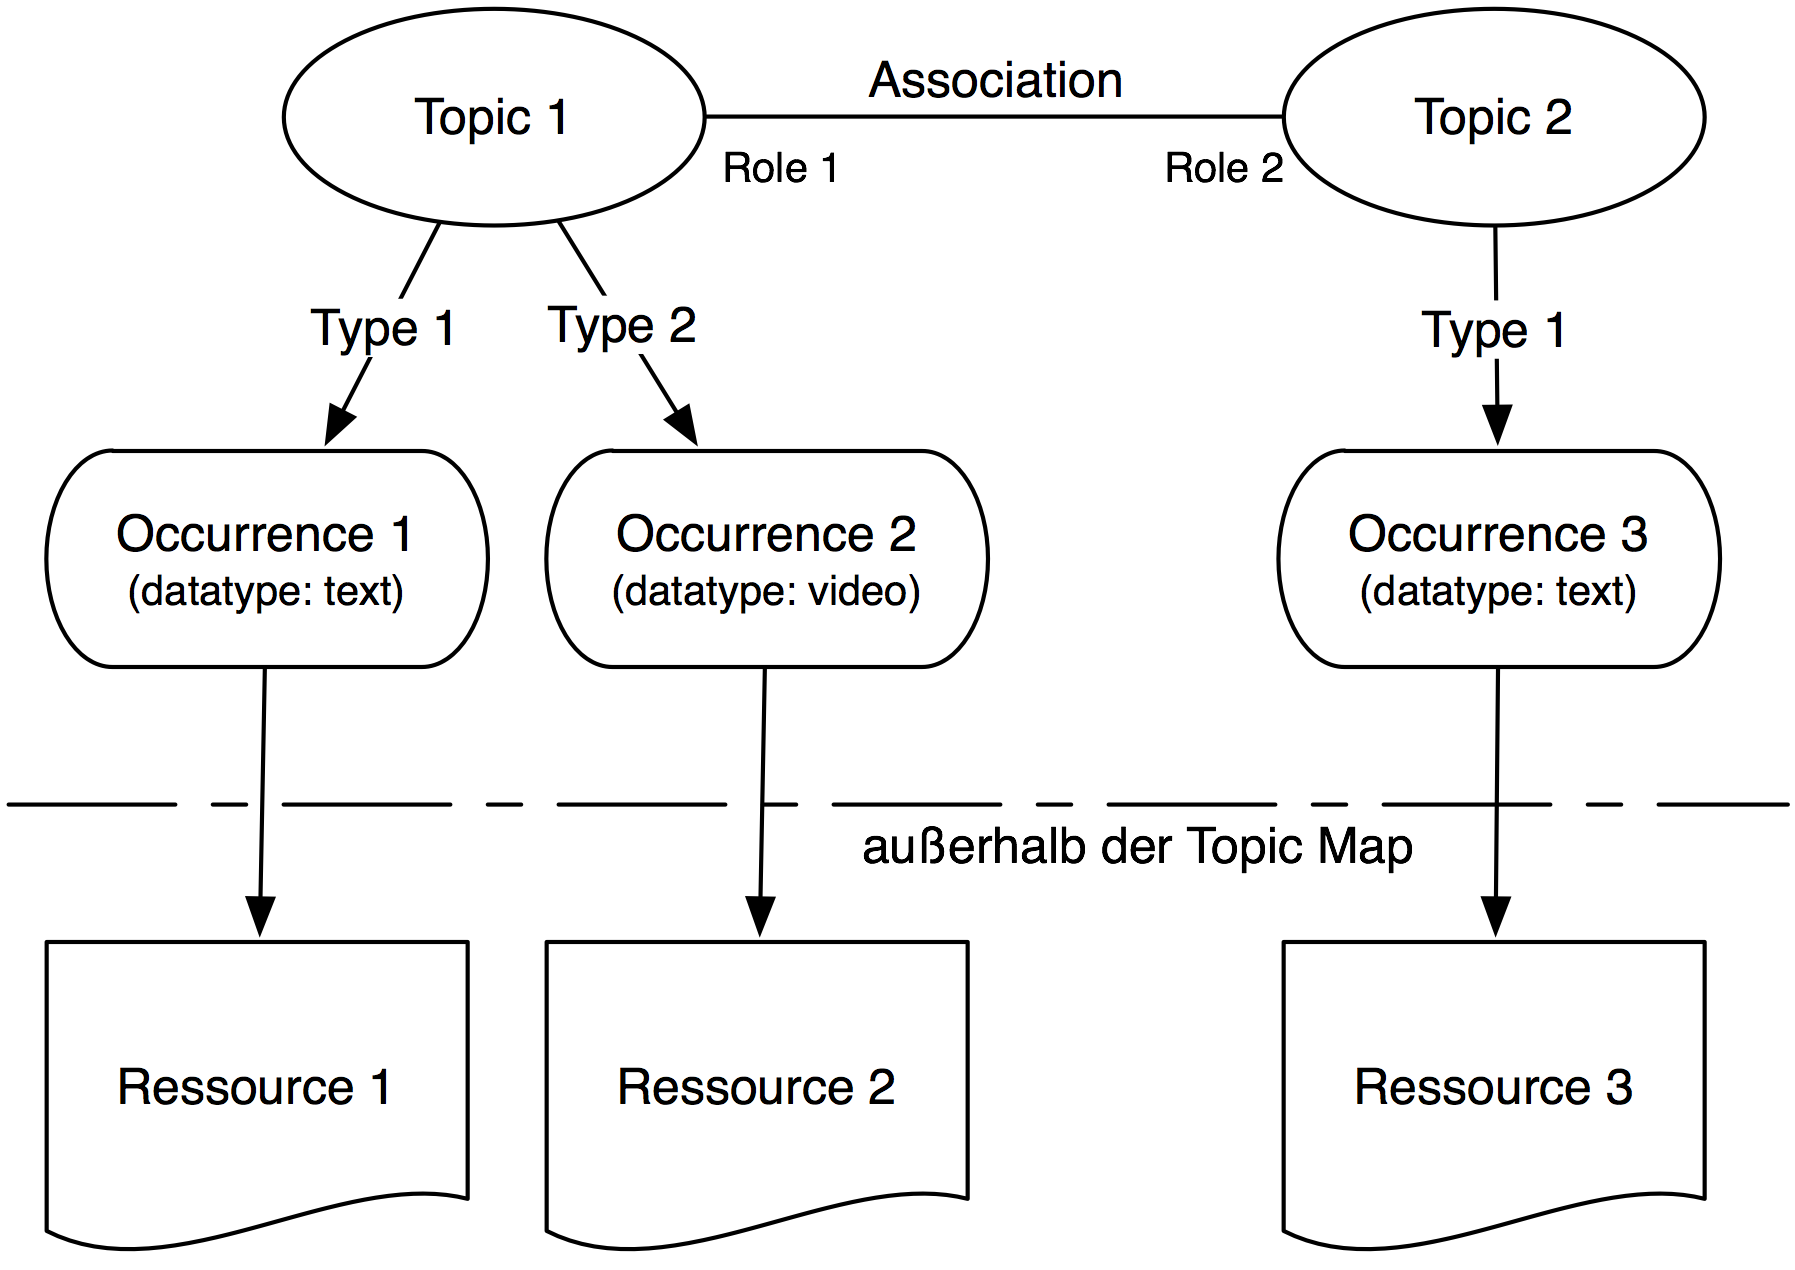
\includegraphics[width=10cm]{img/Persistenz/TMBasic.png}
	\caption{Grundlegende Elemente einer Topic Map}
	\label{fig:img_Persistenz_TMBasic}
\end{figure}

„Topics“ sind stellen Begriffe dar und bilden die Knoten des semantischen Netzes. Ein Topic kann beliebige Information darstellen, repräsentiert aber immer genau ein Phänomen der realen Welt (d.h. zu einem Topic muss es eine Entsprechung außerhalb der Topic Maps geben, die beobachtbar oder beschreibbar ist und auf die die modellierende Person Bezug nehmen will \footnote{„A subject can be anything whatsoever, regardless of whether it exists or has any other specific characteristics, about which anything whatsoever may be asserted by any means whatsoever. In particular, it is anything about which the creator of a topic map chooses to discourse.“ \citep[][S.8]{TMDM08}}). Eine Topic Map ist damit im Sinne von \citet{Stachowiak73} ein diagrammatisches Modell, das einen bestimmten, für den Modellersteller relevanten Ausschnitt der Realität abbildet.

"Associations" bilden die Beziehungen zwischen Topics ab und stellen damit die Kanten des semantischen Netzes dar. Eine Association verknüpft Topics semantisch miteinander und kann frei mit Bedeutung belegt werden. Die Art der Beziehungen ist also nicht festgelegt und wird wie die Bedeutung der Topics frei gewählt werden. Topics und Associations decken historisch den Bereich der Darstellung von Thesauri ab, in denen Begriffe definiert und zueinanden in Beziehung gesetzt werden. 

Der zweite historische Ursprung von Topic Maps, die Indizes, werden durch das Konstrukt der "Occurences" abgedeckt. Occurences ("Auftreten") sind Referenzen aus der Topic Map in die reale Welt. Sie setzen die Topics einer Topic Map in Bezug zu beliebiger referenzierbarer Information (z.B. Dokumente). Im Kontext der eben genannten Indizes, kann eine Topic Map als der mit Querverweisen versehene Index eines Buches verstanden werden, in dem durch die Angabe von Seitenzahlen auf den Text des Buches verwiesen wird. Diese Verweise durch Angabe der Seitenzahlen sind in diesem Zusammenhang die Occurrences.

Die Ansammlung von durch Associations verknüpften und mit Occurrences versehenen Topics bilden eine Topic Map. Darüber hinaus kann in Topic Maps jedoch noch weiterführende Information repräsentiert werden (siehe Abbildung \ref{fig:img_Persistenz_TMFull}), die Gegenstand der folgenden Abschnitte sein werden.

\begin{figure}[htbp]
	\centering
		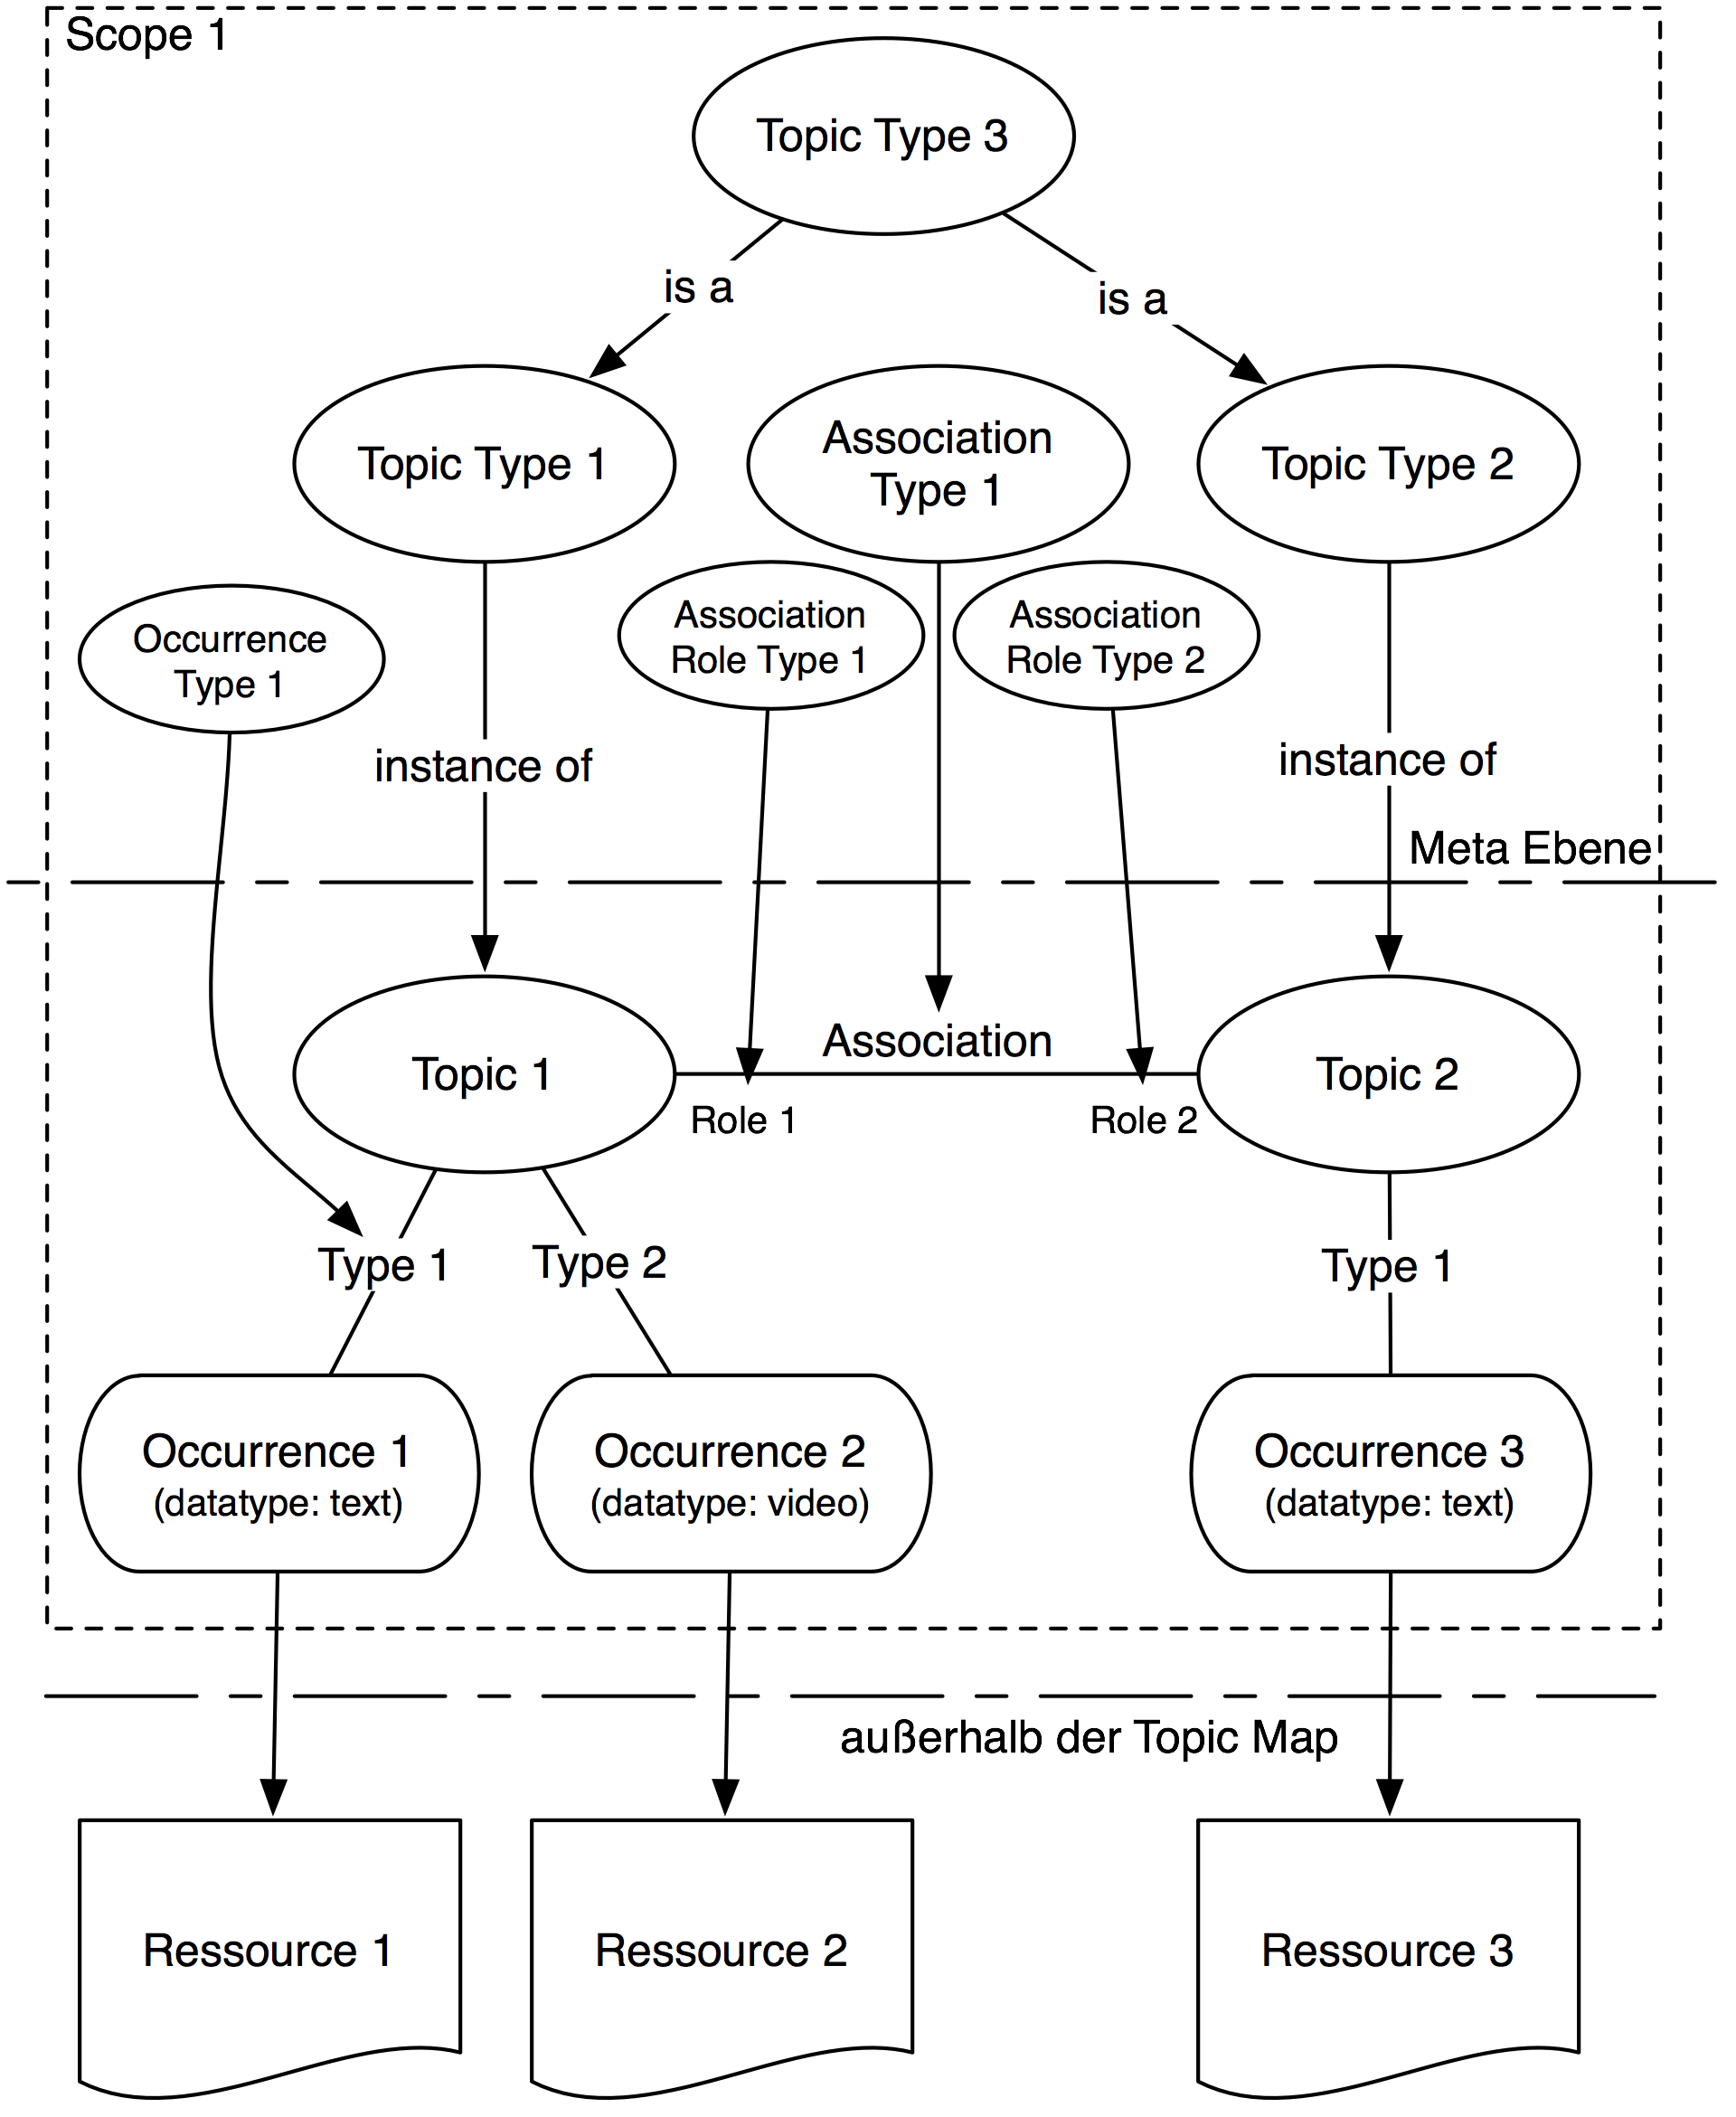
\includegraphics[width=10cm]{img/Persistenz/TMFull.png}
	\caption{Umfassende Darstellung der Elemente einer Topic Map}
	\label{fig:img_Persistenz_TMFull}
\end{figure}

\subsection{Topics, Subjects, Topic Names und Variants} % (fold)
\label{sub:topics_subjects_topic_names_und_variants}

Dieser

\begin{figure}[htbp]
	\centering
		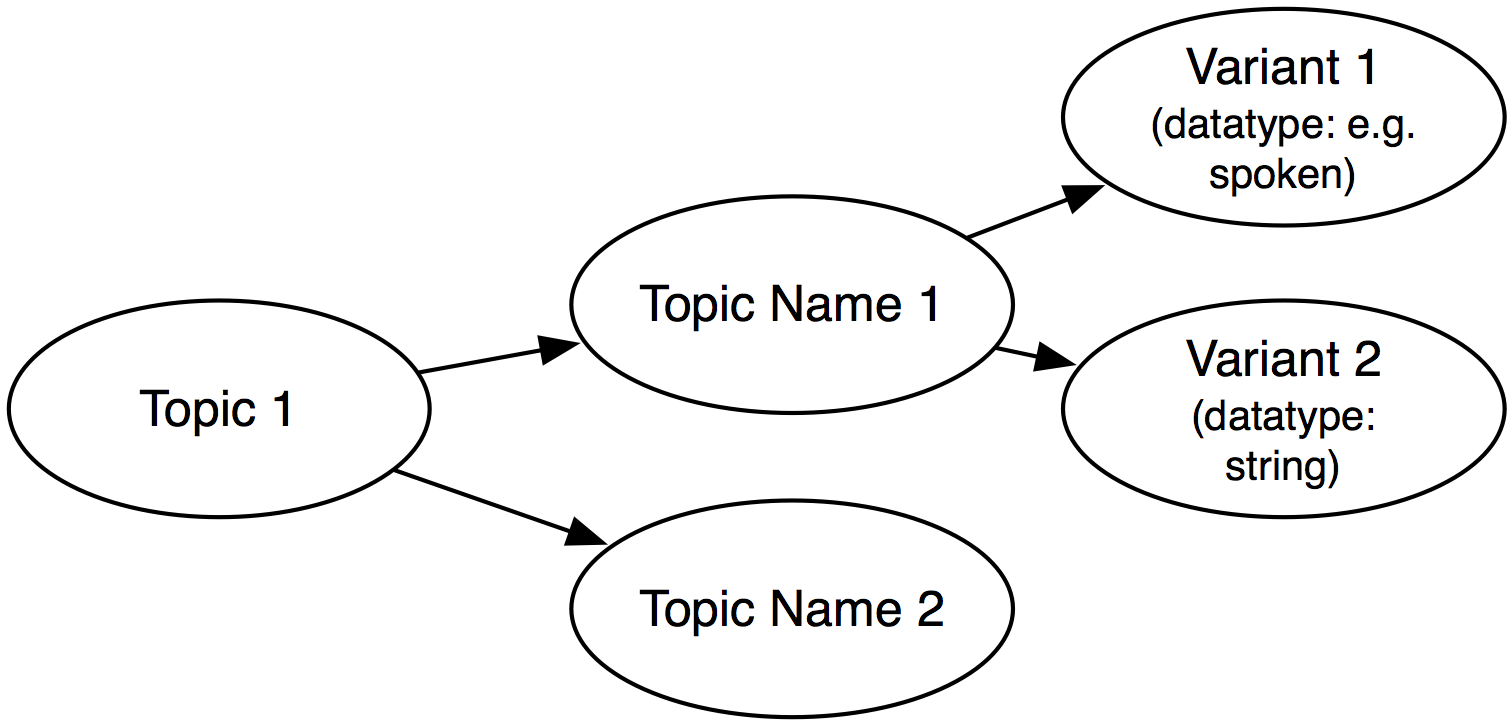
\includegraphics[width=10cm]{img/Persistenz/TopicNaming.png}
	\caption{Benennung von Topics}
	\label{fig:img_Persistenz_TopicNaming}
\end{figure}


% subsection topics_subjects_topic_names_und_variants (end)

\subsection{Associations und Roles} % (fold)
\label{sub:associations_und_roles}

% subsection associations_und_roles (end)

\subsection{Occurrences und Datatypes} % (fold)
\label{sub:occurrences_und_datatypes}

% subsection occurrences_und_datatypes (end)

\subsection{Metamodellierung in Topic Maps} % (fold)
\label{sub:metamodellierung_in_topic_maps}

Topic Types, Association Types und Occurrence Types

\begin{figure}[htbp]
	\centering
		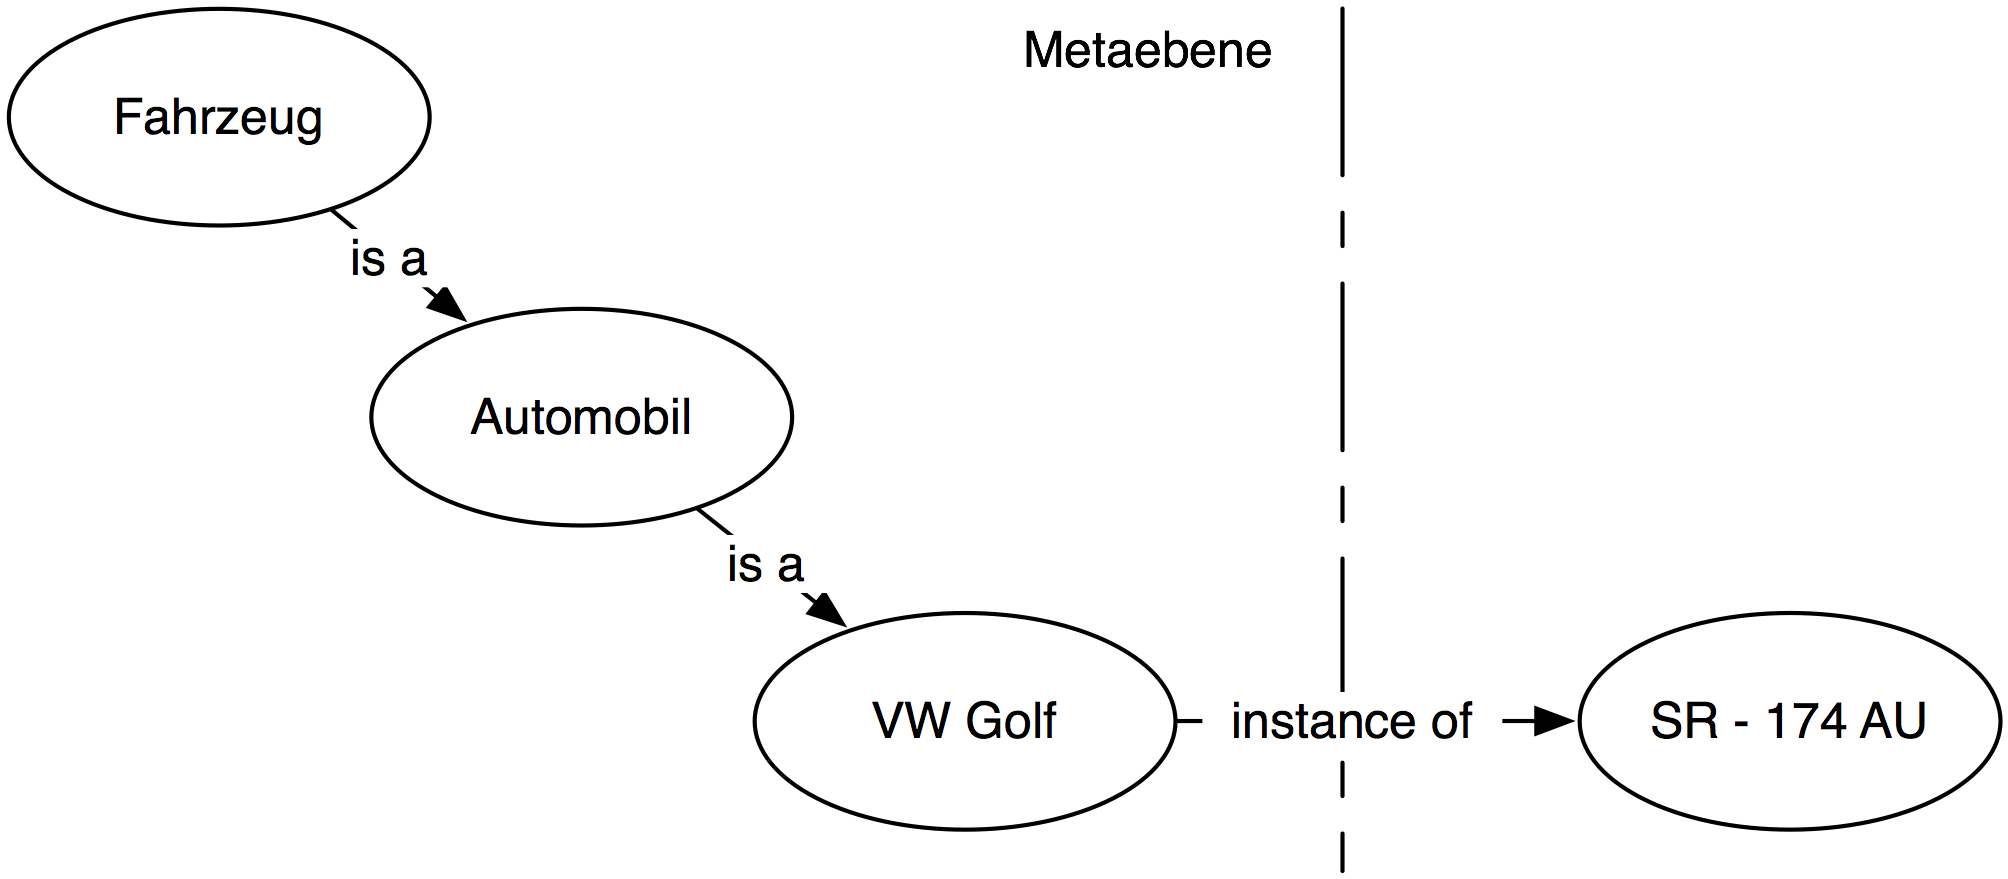
\includegraphics[width=10cm]{img/Persistenz/MetaModelExample.png}
	\caption{Beziehungen in der Metamodellbildung in Topic Maps}
	\label{fig:img_Persistenz_MetaModelExample}
\end{figure}

% subsection metamodellierung_in_topic_maps (end)

\subsection{Scopes} % (fold)
\label{sub:scopes}

% subsection scopes (end)

\subsection{Weiterführende Konzepte} % (fold)
\label{sub:tm_weiterführend}

\subsubsection{Reification} % (fold)
\label{ssub:reification}

% subsubsection reification (end)

\subsubsection{Merging} % (fold)
\label{ssub:merging}

% subsubsection merging (end)
% subsection tm_weiterführend (end)

\subsection{Einschränkungen} % (fold)
\label{sub:einschränkungen}

Regeln und verbindliche Strukturvorgaben
Datenhaltung und Abfrage
% subsection einschränkungen (end)
% section topic_maps (end)

\section{Abbildung von Modellen auf Topic Maps} % (fold)
\label{sec:abbildung_von_modellen_auf_topic_maps}
-> DA Matthias
% section abbildung_von_modellen_auf_topic_maps (end)

\section{Technische Umsetzung der Persistierung von Modellen} % (fold)
\label{sec:technische_umsetzung_der_persistierung_von_modellen}
Topic Map Engine Persistence Layer
% section technische_umsetzung_der_persistierung_von_modellen (end)

\section{Zusammenfassung} % (fold)
\label{sec:persistierung_zusammenfassung}

% section persisitierung_zusammenfassung (end)
% chapter persistierung (end)
